\label{algrothim_description}

The search algorithm which was chosen was the Nelder-Mead search algorithm \cite{nelder_1965}.  This method was selected because it is one of the most popular direct search methods for minimization of functions.  The Nelder-Mead approach is a local optimization search which does not rely on knowledge of the gradient to select the next search point.  This is critical for the application to simulation results because the gradient is unknown and finding it would involve running a large number of simulations.  With simulation times that can reach into days long, this is a critical consideration.  
Instead of knowing the actual function, it relies on n+1 vertices.  This means that a smaller number of simulation runs are needed to perform the minimization \cite{wang_2011}.
The flow chart in Figure \ref{fig:nm_flow} is the flow which is used to determine the next search point.
\begin{figure}[!htb]
	\centering
	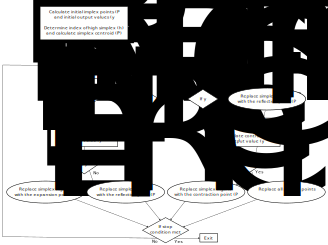
\includegraphics[width=\textwidth]{nm_flow}
	\caption{Flow chart for the Nelder-Mead search algorithm\cite{nelder_1965}}
	\label{fig:nm_flow}
\end{figure}

In general, for each time step the reflection point is calculated using Equation \ref{eqn:reflection} where $\alpha$ is the reflection coefficient.
	\begin{equation}\label{eqn:reflection}
		P_{refl} = (1 + \alpha) P_{cent} - \alpha P_{high}
	\end{equation}
If this reflection point is smaller than the smallest current simplex value, then the expansion is calculated using Equation \ref{eqn:expansion}, where $\gamma$ is the expansion coefficient.
	\begin{equation}\label{eqn:expansion}
		P_{exp} = \gamma P_{refl} - (1 - \gamma) P_{center}
	\end{equation}
If the expansion point is smaller than the reflection point, then the expansion point is used to replace the largest simplex member.  Otherwise, if the reflection point is larger than the expansion point, the reflection point is used to replace the largest member of the simplex, and the algorithm is restarted.
If the reflection point is larger than the smallest simplex point and smaller than the second largest point, then the highest point of the simplex is replaced with the reflection and the algorithm is restarted. 
If the reflection point is between the simplex high and second highest value, a contraction is calculated, using Equation \ref{eqn:reflection}, with the highest values being replaced with the reflection.  Otherwise the contraction is calculated with the original simplex still using Equation \ref{eqn:reflection}, where $\beta$ is the contraction coefficient.
	\begin{equation}\label{eqn:contraction}
		P_{cont} = \beta P_{high} - (1 - \beta) P_{cent}	
	\end{equation}
If the contraction point is smaller than the largest point of the simplex, then the contraction replaces the largest point and the algorithm is continued.
However if the contraction point is larger than the highest point, a shrink step is performed, detailed in Equation \ref{eqn:shrink}, where $\delta$ is the shrink coefficient and the algorithm is restarted.
	\begin{equation}\label{eqn:shrink}
		P_{i} = \delta P_{i} + (1 - \delta) P_{low}
	\end{equation}